\documentclass[a4paper,14pt]{article}

\usepackage{comment} % Para comentar várias linhas ao mesmo tempo

%matemática
\usepackage{amsmath}
\usepackage{amssymb}

%diagramação
\usepackage{extsizes}
\everymath{\displaystyle}
\usepackage{geometry}
\usepackage{fancyhdr}
\usepackage{multicol}
\usepackage{graphicx}
\usepackage[brazil]{babel}
\usepackage[shortlabels]{enumitem}
\usepackage{cancel}
\usepackage{textcomp}
\usepackage{tcolorbox}

%tabelas
\usepackage{array} % Para melhor formatação de tabelas
\usepackage{longtable}
\usepackage{booktabs}  % Para linhas horizontais mais bonitas
\usepackage{float}   % Para usar o modificador [H]
\usepackage{caption} % Para usar legendas em tabelas
\usepackage{wrapfig} % Para usar tabelas e figuras flutuantes
\usepackage{xcolor} % Para cores do fundo de tabelas
\usepackage{colortbl} % Para cores do fundo de tabelas

%tikzpicture
\begin{comment}
	\usepackage{tikz}
	\usepackage{scalerel}
	\usepackage{pict2e}
	\usepackage{tkz-euclide}
	\usetikzlibrary{calc}
	\usetikzlibrary{patterns,arrows.meta}
	\usetikzlibrary{shadows}
	\usetikzlibrary{external}
\end{comment}


%pgfplots
\usepackage{pgfplots}
\pgfplotsset{compat=newest}
\usepgfplotslibrary{statistics}
\usepgfplotslibrary{fillbetween}

%colours
\usepackage{xcolor}



\columnsep=2cm
\hoffset=0cm
\textwidth=8cm
\setlength{\columnseprule}{.1pt}
\setlength{\columnsep}{2cm}
\renewcommand{\headrulewidth}{0pt}
\geometry{top=1in, bottom=1in, left=0.7in, right=0.5in}

\pagestyle{fancy}
\fancyhf{}
\fancyfoot[C]{\thepage}

\begin{document}
	
	\noindent\textbf{6FMA133 - Matemática} 
	
	\begin{center}Redução percentual (Versão estudante)
	\end{center}
	
	\noindent\textbf{Nome:} \underline{\hspace{10cm}}
	\noindent\textbf{Data:} \underline{\hspace{4cm}}
	
	%\section*{Questões de Matemática}
	
	\begin{multicols}{2}
	    \noindent Suponha que um valor $y$ foi reduzido de $x\%$.
	    \begin{itemize}
	    	\item Para sabermos o valor da redução, devemos fazer: \\\\ $\frac{x}{100} \cdot y$ $\longrightarrow$ valor reduzido
	    	\item Para sabermos o valor final, após a redução, devemos fazer: \\\\ $\frac{100 - x}{100} \cdot y$ $\longrightarrow$ valor final
	    \end{itemize}
		\noindent\textsubscript{--------------------------------------------------------------------------}
		\begin{enumerate} 
			\item Um carro custa R\$ 56.000,00. Foi anunciado que esse carro terá um desconto de 2,3\% em seu preço. Quanto ele irá custar? \\\\\\\\\\\\\\\\\\\\\\\\\\\\\\\\\\
			\item Em 2018, havia 72 500 habitantes em uma certa idade. No ano seguinte, calculou-se que houve um aumento percentual de 7\% na população dessa cidade. Qual o número de habitantes em 2019? \\\\\\\\\\\\\\\\\\\\
			\item O preço de um livro em dezembro era R\$ 70,00. Em janeiro, estava custando R\$ 56,00. Em quantos por cento, diminuiu seu preço? \newpage
			\item Uma pessoa comprou um terreno com desconto de 40\% sobre o seu preço normal, que é de R\$ 130.000,00. Em seguida, vendeu-o por um preço 60\% maior do que pagou. Por quanto vendeu o terreno? \\\\\\\\\\\\\\\\
			\item Uma loja anunciou que venderia um modelo de geladeira, vendido normalmente a 2 600 reais com desconto de 45\% para pagamento à vista a partir de um certo dia. No dia anterior ao início do desconto, porém, a loja aumentou o preço da geladeira, de forma que, com desconto, custaria exatamente o preço normal de 2 600 reais. Em quantos por cento, aproximadamente, foi aumentado o preço nessa manobra comercial? \\\\\\\\\\\\\\\\\\\\\\\\
			\textbf{Desafio olímpico} \\\\
			(OBMEP) O gráfico representa o percentual de aumento do preço de dois produtos, $A$ e $B$, em uma mercearia no primeiro e no segundo semestres do ano passado. As afirmativas abaixo referem-se ao período completo do ano passado. Qual delas é a correta? \\
			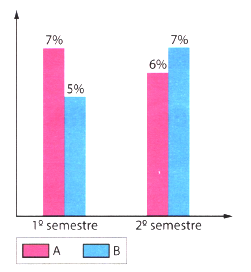
\includegraphics[width=1\linewidth]{6FMA133_imagens/imagem1}
			\begin{enumerate}[a)]
				\item O aumento percentual do preço de $B$ foi maior do que o de $A$.
				\item O aumento percentual do preços dos dois produtos foi o mesmo.
				\item O aumento percentual do preço de $A$ foi de exatamente 13\%.
				\item O preço de $A$ diminuiu e o de $B$ aumentou.
				\item O aumento percentual do preço de $B$ foi maior do que 12\%.
			\end{enumerate}
			\newpage
			%33 a 36
			\item Uma loja está em promoção e diminuiu todos os seus preços em 15\%. Júlio comprou cinco blusas cujo preço antes da promoção era R\$ 65,00 cada uma. Quanto Júlio pagou pelas blusas? \\\\\\\\\\\\\\\\\\\\\\\\\\\\
			\item Uma joalheria lançou uma promoção diferente: diminuiu todos os seus preços em R\$ 12,00.
			\begin{enumerate}[a)]
				\item Alexandre vai se casar e foi a essa joalheria comprar uma aliança cujo preço era R\$ 160,00. Em quantos por cento o preço da aliança diminuiu? \\\\\\\\\\\\\\\\\\\\\\
				\item Renato resolveu comprar lá uma corrente e pagou R\$ 208,00. Em quantos por cento, aproximadamente, o preço da corrente tinha diminuído? \\\\\\\\\\\\\\\\\\\\\\
				\item O senhor Carlos viu uma bela moeda de prata e resolveu comprá-la. A moeda custava R\$ 92,00 antes da promoção. Ao ver o preço, o senhor Carlos negociou com o gerente da loja, conseguindo um desconto de 30\% sobre o preço da promoção. Dias depois, ele vendeu a moeda por R\$ 98,00. Qual foi a porcentagem de lucro do senhor Carlos? \\\\\\\\\\\\\\\\\\\\\\
			\end{enumerate}
			\item Um comerciante decidiu aumentar seus preços em 25\%. Após um tempo, sem ter aumento em suas vendas, ele anunciou um desconto de 25\% em todas as suas peças. Qual foi a variação sofrida pelos preços em termos de valores originais? \\\\\\\\\\\\\\\\\\\\\\
			\item Na loja de Patrícia, o preço de um livro foi diminuindo em 60\%. Em que porcentagem Patrícia deve aumentar o preço diminuído para que, com o aumento, o novo preço do livro coincida com o original?
		\end{enumerate}
		$~$ \\ $~$ \\ $~$ \\ $~$ \\ $~$ \\ $~$ \\ $~$ \\ $~$ \\ $~$ \\ $~$ \\ $~$ \\ $~$ \\ $~$ \\ $~$ \\ $~$ \\ $~$ \\ $~$ \\ $~$ \\ $~$ \\ $~$ \\ $~$ \\ $~$ \\ $~$ \\ $~$ \\ $~$ \\ $~$ \\ $~$ \\ $~$ \\ $~$ \\ $~$ \\ $~$ \\ $~$ \\ $~$ \\ $~$ \\ $~$ \\ $~$ \\ $~$ \\ $~$ \\ $~$ \\ $~$ \\ $~$ \\ $~$ \\ $~$ \\ $~$ \\ $~$ \\ $~$ \\ $~$ \\ $~$ \\ $~$ \\ $~$ \\ $~$ \\ $~$ \\ $~$ \\ $~$ \\ $~$ \\ $~$ \\ $~$
	\end{multicols}
\end{document}